% !TEX root = ../thesis_main.tex
\chapter{Experimental Procedures}


\section{Introduction}

This chapter presents all relevant procedures used to conduct this study. In particular, Section \ref{section:cnt_synthesis} gives a brief review of the techniques used to synthesis the SWCNTs used for sample preparation. Furthermore, Sections \ref{sec:aqueous_susp} and \ref{sec:polymer_susp} describe the procedures used in making the (6,5)-enriched SWCNT aqeuous suspenion as well as the (6,5)-enriched polymer-wrapped suspension, respectively, that were studied. Finally, Section \ref{sec:experimental_proced} reports the methods used in collecting the experimental data.

\section{Synthesis of SWCNTs}
\label{section:cnt_synthesis}
Catalytic chemical vapor deposition (CCVD) is a standard method for synthesizing carbon nanotubes (CNTs) \cite{prasek2011methods, agboola2007conceptual}. This technique depends on the decomposition of carbon sources, such as methane and acetylene, via heat or plasma irradiation to form carbon nanotubes on a substrate \cite{agboola2007conceptual}. Such reactions are typically driven by transition-metal catalysts such as nickel, iron, and cobalt \cite{prasek2011methods}.

One commonly used process known as the CoMoCAT method involves catalytic reactions that include cobalt (Co) and molybdenum (Mo) as catalysts \cite{resasco2002scalable}. Here, carbon monoxide gas (CO$_\text{(g)}$) is used as a carbon source that decomposes in the reaction
\vspace{-2mm}
\begin{equation}
\label{eq:cnt_synth}
\ce{CO_{(g)} + CO_{(g)} $\rightarrow$ CO_2_{\text{(g)}} + C_{(CNT)}},
\end{equation}
to form carbon nanotubes \cite{resasco2002scalable}. This process is typically conducted at temperatures between 700 and \SI{900}{\celsius} and pressures ranging from 1 $-$ 10 atm \cite{resasco2002scalable}.

Another well-known technique, commonly referred to as the HiPco method, involves the use of high-pressure carbon monoxide \cite{bronikowski2001gas, nikolaev1999gas}. This process takes place inside a furnace at temperatures as high as 900 $-$ \SI{1100}{\celsius} and at high pressures between 30 and 50 atm. Synthesis occurs by flowing carbon monoxide gas along with iron pentacarbonyl (Fe(CO)$_5$) into the furnace \cite{nikolaev1999gas}. The Fe(CO$_5$) molecules decompose to form gas-phase iron clusters upon which the chemical reaction defined in Equation \eqref{eq:cnt_synth} occurs. It is well understood that the CoMoCAT and HiPco methods both produce an ensemble of nanotubes with varying chiralities \cite{agboola2007conceptual}. As such, these ensembles are often used as precursor materials for filtration techniques capable of creating dispersions that are enriched by a single chirality \cite{janas2018towards, zheng2019sorting}.

\begin{figure}[ht]
	\centering
	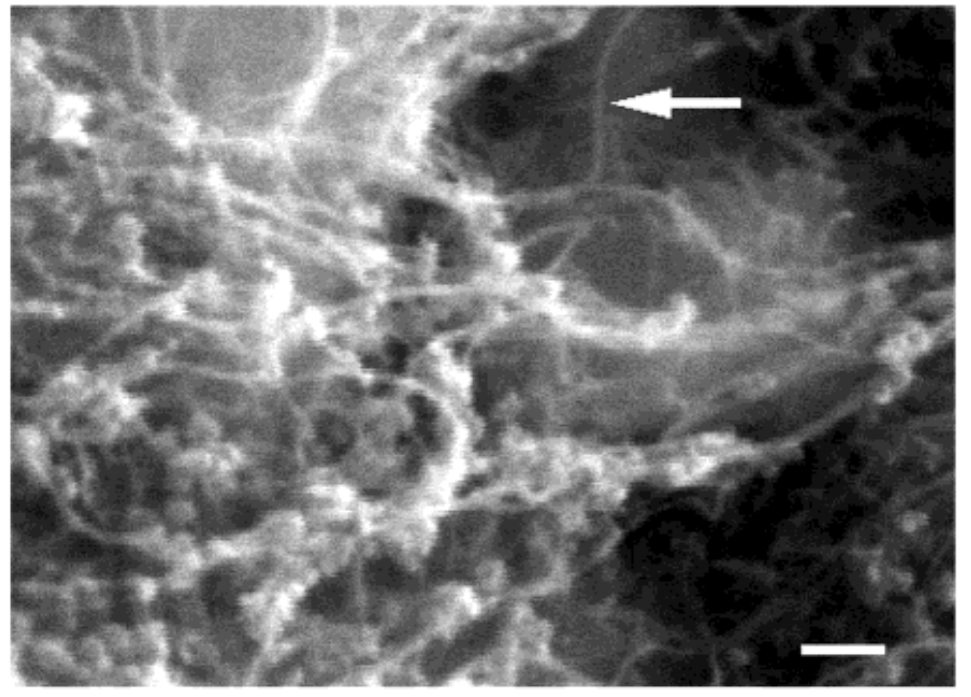
\includegraphics[scale=0.3]{images/chapter_methods/sem_cnt_powder_bandy}
	\caption{(a) Scanning electron microscope image of as-produced nanotube powder. The scale bar corresponds to a length scale of 200 nm. The arrow indicates a single rope emerging out of the nanotube bundle. Reproduced from Ref.\ \cite{bandyopadhyaya2002stabilization}.}
	\label{fig:cnt_powder}
\end{figure}


In this powdered form shown in Figure \ref{fig:cnt_powder}, SWCNTs have a tendency to form ropes and bundles due to strong van der Waals interactions as high as \SI{500}{\electronvolt / \micro \meter} between nanotubes \cite{thess1996crystalline, girifalco2000carbon}. Such interactions between nanotubes can have the effect of broadening optical resonances, making it harder to distinguish between chirality-dependent features \cite{liu1998fullerene, o2001reversible, o2002band}, as shown in Figure \ref{fig:cnt_dispersion_vs_rope}. For instance, if metallic and semiconducting nanotubes are in electronic contact, this would give carriers generated in semiconducting nanotubes an intraband relaxation pathway through the gapless, continuum states of metallic nanotubes \cite{ostojic2004interband}.



\begin{figure}[H]
	\centering
	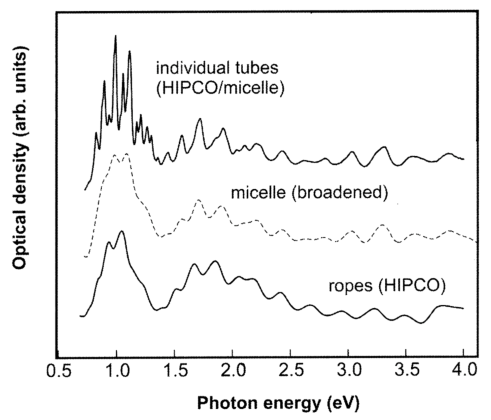
\includegraphics[scale=1.]{images/chapter_methods/cnt_rope_vs_micelle}
	\caption{Optical absorption spectra of HiPco carbon nanotubes. The top spectrum shows the optical absorption for an ensemble of individually suspended HiPco nanotubes. The middle spectrum shows the effect of numerically broadening the peaks of the top spectrum. The bottom spectrum shows the optical absorption of a HiPco nanotube bundle. Due to intertube interactions, the optical resonances of the HiPco bundle become severely broadened, making it hard to distinguish between chirality-dependent features. For a individually suspended SWCNTs, these resonances are more easily observed. Reproduced and modified from Ref.\ \cite{hagen2003quantitative}.}
	\label{fig:cnt_dispersion_vs_rope}
\end{figure}

\section{Preparation of the Studied (6,5)-enriched SWCNT Aqueous Suspension}
\label{sec:aqueous_susp}

\subsection{Overview}
In this section, we review the technique used to prepare the aqueous suspension of (6,5)-enriched SWCNTs. In brief, HiPCo SWCNTs were first dispersed in an aqueous solution containing sodium dodecyl sulfate (SDS) and sodium cholate (SC) using sonication followed by ultracentrifugation. We then performed gel chromtagraphy on this SWCNT suspension to create a (6,5)-enriched SWCNT suspension. In the final steps, the SDS and SC surfactants were later removed using a filter membrane and the SWCNTs were again redispersed using sodium deoxy-cholate (DOC).

\subsection{Dispersion of SWCNTs by Sonication}
\label{section:dispersion_swcnt}
We created an aqeuous suspension of (6,5)-enriched sample by starting with CoMoCAT SWCNTs obtained from Sigma-Aldrich (Manufacturer Number: Signis$^{\tiny{\textregistered}}$ SG65i). This initial product consisted of a powder of SWCNTs with an average diameter of 0.78 nm and a median length of \SI{1}{\micro \meter}. Approximately 95\% of the SWCNTs are semiconducting with 41\% of them being (6,5) SWCNTs.


First, we dispersed CoMoCAT SWCNTs in an aqueous solution containing surfactants by using sonication followed by ultracentrifugation \cite{liu1998fullerene, o2001reversible, o2002band}. Sonication uses mechanical vibrations to break up the van der Waals interactions that hold nanotube bundles together . Furthermore, the presence of surfactant molecules has the effect of mitigating inter-tube interactions to stabilize the suspension by preventing the formation of nanotube bundles \cite{liu1998fullerene, o2001reversible, o2002band}.

\begin{figure}[H]
\centering
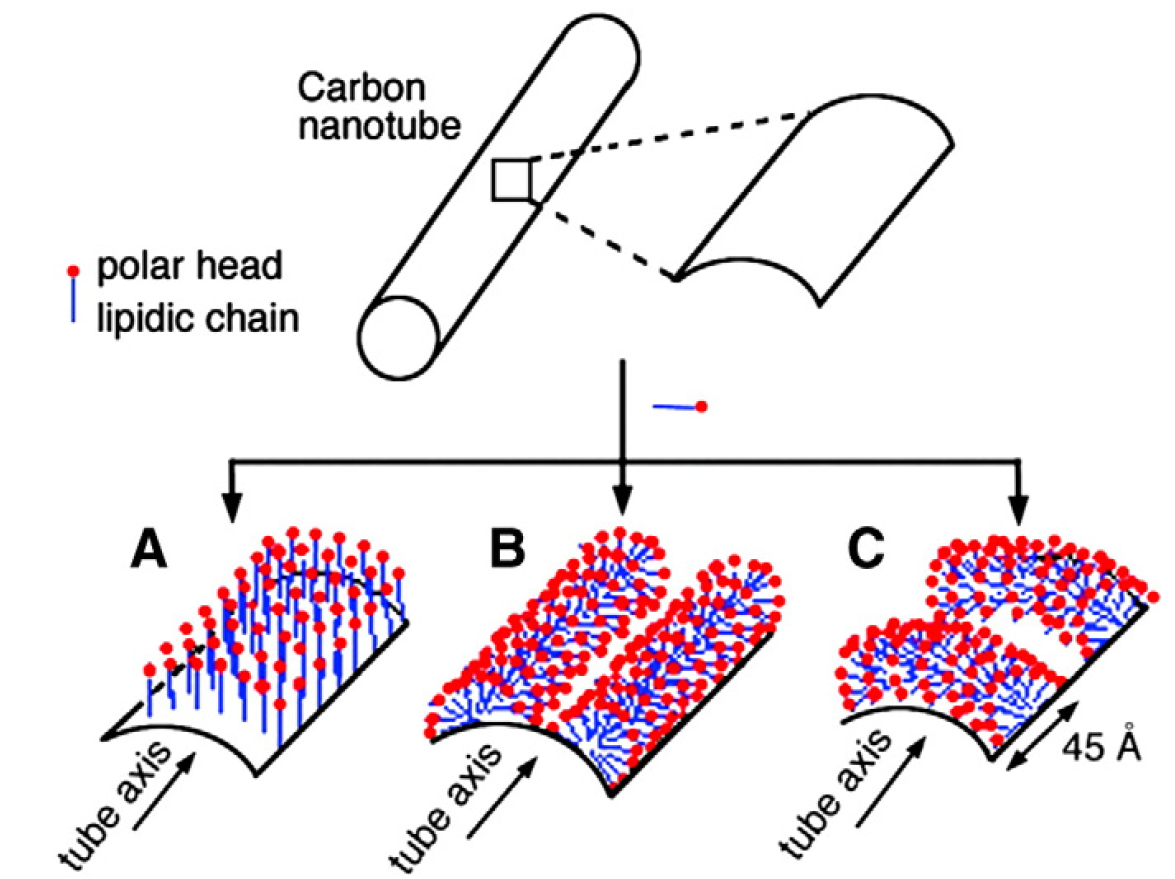
\includegraphics[scale=0.3]{images/chapter_methods/surfactant_tkalya}
\caption{Surfactants such as sodium dodecyl sulfate (SDS) can become adsorbed on the surfaces of SWCNTs in three ways. (A) Adsorbed SDS molecules form a monolayer on the nanotube surface. In addition, adsorbed SDS molecules can form half-cylinders on the surface of nanotubes that are (B) aligned parallel to the tube axis or (C) aligned perpendicular to the tube axis. Reproduced from Ref.\ \cite{richard2003supramolecular}. }
\label{fig:sds_molecule}
\end{figure}

SDS represents an exemplary surfactant commonly used to prepare dispersions of carbon nanotubes. In the aqeuous dispersion, SDS molecules become adsorbed on the outer surface of the nanotubes, as shown in Figure \ref{fig:sds_molecule}. Here, the hydrophobic part of SDS becomes adsorbed onto the nanotube surface while the hydrophilic part points towards the aqueous phase and aids with the dissolution of the nanotube \cite{richard2003supramolecular}. This forms a distribution of negative charge on nanotube surfaces due to the negatively-charged hydrophilic region that, via Coulomb interactions, prevents nanotubes from sustaining physical contact \cite{richard2003supramolecular}.


Unfortunately, not all nanotube bundles can be broken up by sonication \cite{o2002band}. Therefore, ultracentrifugation is used to separate dispersed nanotubes from the remaining bundles \cite{o2002band}. This yields a mixture composed of nanotubes floating in the aqeuous solution above a sediment of nanotube bundles. We then extracted the aqeuous solution containing the dispersed nanotubes, also known as the supernatant, and performed gel chromatography on this product to obtain a (6,5)-enriched sample.

\subsection{SWCNT Chirality Enrichment by Gel Chromatography}

Gel chromatography works by separating nanotubes according to their relative diameters \cite{liu2011large}. Figure \ref{fig:gel_chromatography_kataura} shows a schematic diagram of how this method works. By exploiting the fact that certain chiralities will interact more strongly with the gel than others, chirality-enriched suspensions can be readily prepared.

The gel chromatography procedure we used was devised by Ichinose \textit{et al}. \cite{ichinose2017extraction}. First, the CoMoCAT SWCNTs are dispersed in an aqeuous solution containing the surfactants sodium dodecyl sulfate (SDS) and sodium cholate (SC) with concentrations of 0.5\% each. This dispersion is then placed in a column containing hydrogel beads at the bottom. Depending on the pH of the aqueous solution, some SWCNTs become more readily adsorbed onto the hydrogels, making it easy to filter out those that are not adsorbed \cite{liu2011large}. Here, the pH of the solution is controlled via carbon dioxide bubbling \cite{ichinose2017extraction}. As shown in Figure \ref{fig:elute_ph}, nanotubes such as (8,6) and (11,1) can be removed (eluted) when the pH is set to 8.1 \cite{ichinose2017extraction}. By progressively reducing the pH in increments of 0.1, other unwanted chiralities such as (7,6) can now be eluted until only (6,5) nanotubes remain \cite{ichinose2017extraction}.

\begin{figure}[H]
	\centering
	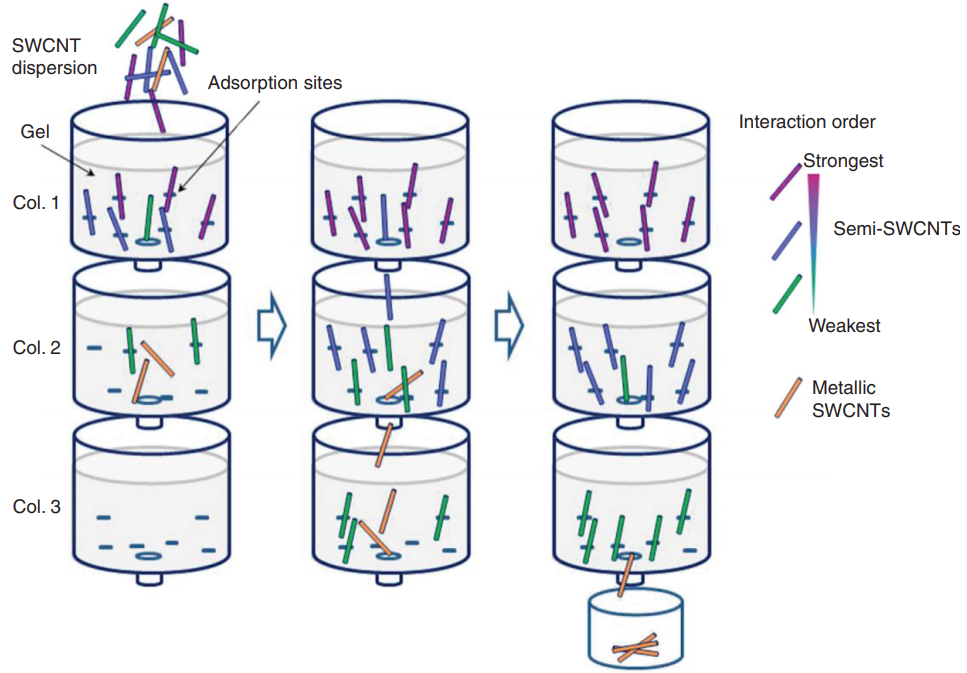
\includegraphics[scale=1.7]{images/chapter_methods/multi_column_kataura}
	\caption{SWCNT chiralty separation using multicolumn single-surfactant gel chromatography. This technique employs a series of connected columns, each containing an allyl dextran-based gel. By exploiting the tendency of SWCNTs that interact more strongly with the gel will be held within a limited set of adsorption sites, and the remaining SWCNTs will pass through into the next column. It has been observed that semiconducting nanotubes tend to interact more strongly with the gel than metallic nanotubes. This makes it possible to create ensembles enriched by either semiconducting or metallic nanotubes. Reproduced from Ref. \cite{liu2011large}.}
	\label{fig:gel_chromatography_kataura}
\end{figure}

In the final steps, the (6,5)-enriched dispersion is dispersed using DOC after removing the SDS and SC from solution. \footnote{As an aside, these samples are often used to make nanotube films. It has been observed that using DOC instead of SC and SDS can yield nanotube films with better alignment. However, at the time of writing, the alignment mechanism has still not been very well understood.} This is accomplished by filtering out SDS and SC using a filter membrane (Amicon$^{\tiny\textregistered}$ Ultra-15 Centrifugal Filter Unit). Afterward, the remaining nanotubes are redispersed using DOC via sonication followed by ultracentrifugation as described in Section \ref{section:dispersion_swcnt}. Now, the sample consists of (6,5)-enriched SWCNTs dispersed in aqueous soltuion containing 4\% concentration of DOC. This mixture is finally pipetted into a quartz cuvette with an optical path length of 1 mm.



\begin{figure}[H]
	\centering
	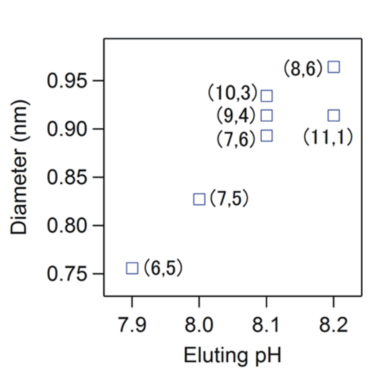
\includegraphics{images/chapter_methods/elute_ph}
	\caption{The plot shows the relationship between the diameters of carbon nanotubes present in the aqeuous solution and the pH required to elute them from the aqueous solution. At a pH set to $8.0$, nanotubes such as (7,5) and (11,1) can be eluted from the mixture whilst (6,5) nanotubes will remain in the solution.  Reproduced from Ref.\ \cite{ichinose2017extraction}.}
	\label{fig:elute_ph}
\end{figure}

\section{Preparation of the Studied Polymer-Wrapped (6,5)-enriched Suspension}
\label{sec:polymer_susp}

\subsection{Overview}
In this section, we review the technique used to prepare the polymer-wrapped suspension of (6,5)-enriched SWCNTs. In brief, CoMoCAT SWCNTs were first dispersed in a toluene solution containing the polymer PFO-BPy (poly[(9,9-dioctylfluorenyl-2,7-diyl)-alt-co-(6,6 0 -\{2,2 0 -bipyridine\})) using shear force mixing. The PFO-BPy polymer itself provided a mechanism for performing chirality enrichment as the SWCNTs were dispersed.

\subsection{Dispersion of SWCNTs by Shear Force Mixing}

The overall procedure for the preparation of the polymer-wrapped (6,5)-enriched suspension used in this study was first reported by Graf \textit{et al}.\ \cite{graf2016large}. The goal of this study was to devise a method capable of preparing chirality-enriched SWCNT suspensions, with a high photoluminescnce quantum yield, at a large scale and in a time-efficient manner. The standard technique of sonicating SWCNT bundles in a solution tends to produce SWCNTs with shorter lengths ($\sim$\SI{1}{\micro\meter}) and a higher presence of lattice defects \cite{khan2010high}, which has been observed to limit the photoluminescence quantum yield of SWCNTs \cite{mouri2012dispersion}. Graf \textit{et al}.\ aimed to devise another method capable of creating suspensions of longer length SWCNTs \cite{graf2016large}.

In their study, they proposed using an alternative method for dispersing SWCNTs, known as shear force mixing (SFM) \cite{hall2011scaling, zhang2012high}. Shear force mixers work differently than conventional mixers. Figure \ref{fig:mixing_paton} shows images of a shear force mixer head and how it works. SFM utilizes a rotor-stator to pump solids and fluids into the head and rely on centrifugal forces to drive the mixture through perforations at the edge of the rotor-stator \cite{paton2014scalable}. This process introduces intense shear forces as the materials are propelled at a high velocity within the head \cite{paton2014scalable}. In general, SFM has traditionally been used in industrial settings for preparing emulsions, dissolving solids, solid-liquid suspensions among other applications \cite{hall2011scaling, zhang2012high}. More recently, it has also been used for research purposes to exfoliate low-dimensional materials such as graphene \cite{paton2014scalable} and molybdenum disulfide \cite{varrla2015large}.



Graf \textit{et al}.\ demonstrated that SFM can produce suspensions of SWCNTs with lengths that are longer than those produced by sonication \cite{graf2016large}. Here, they used CoMoCAT SWCNTs, 40\% of which were (6,5) SWCNTs, to prepare each sample. The surfactant-suspended samples were prepared using SDS in an aqueous solution. Here, they used the standard technique of sonicating the ensemble followed by centrifugation. For the ensemble prepared using SFM, the SWCNTs were dispersed using the polymer PFO-BPy in a toluene solution. The exact motivation for using this polymer is described in the next section.


Figure \ref{fig:dist_graf} shows the length distributions of (6,5)-enriched ensembles prepared using various dispersion methods. The ensemble prepared using SFM had a mean length of \SI{1.82}{\micro\meter}. This was higher than those obtained using dispersed using a sonication bath and tip sonication, which exhibited mean lengths of \SI{1.12}{\micro\meter} and \SI{0.62}{\micro\meter}, respectively. Aside from this, the SFM ensemble also contained SWCNTs that were as long as \SI{5}{\micro\meter}. These were not observed in the ensembles prepared using sonication techniques.

\begin{figure}[H]
	\centering
	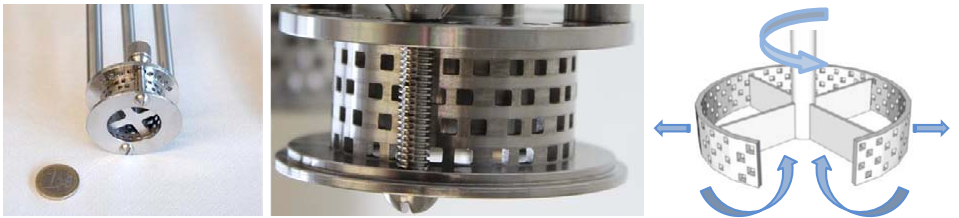
\includegraphics[scale=0.4]{images/chapter_methods/mixing_paton}
	\caption{A close up view of a rotor-stator used for shear force mixing. On the rightmost figure, the top arrow indicates the direction of rotation of the rotor. The perforated screen, known as the stator, remains stationary during operation. The other arrows illustrate the propagation direction of fluid flow. Here, fluids are pumped into the rotor-stator head, and expelled through the perforated screen. In addition, the mixer pictured here has a maximum rotor speed of 8000 rpm and an overall diameter of 50 mm. It also has a small gap between the rotor and stator of \SI{135}{\micro\meter}. The stator itself has 96 perforated holes, each having dimensions of \SI{2}{\milli\meter} $\times$ \SI{2}{\milli\meter}. Reproduced from Ref.\ \cite{paton2014scalable}. }
	\label{fig:mixing_paton}
\end{figure}


\begin{figure}[H]
	\centering
	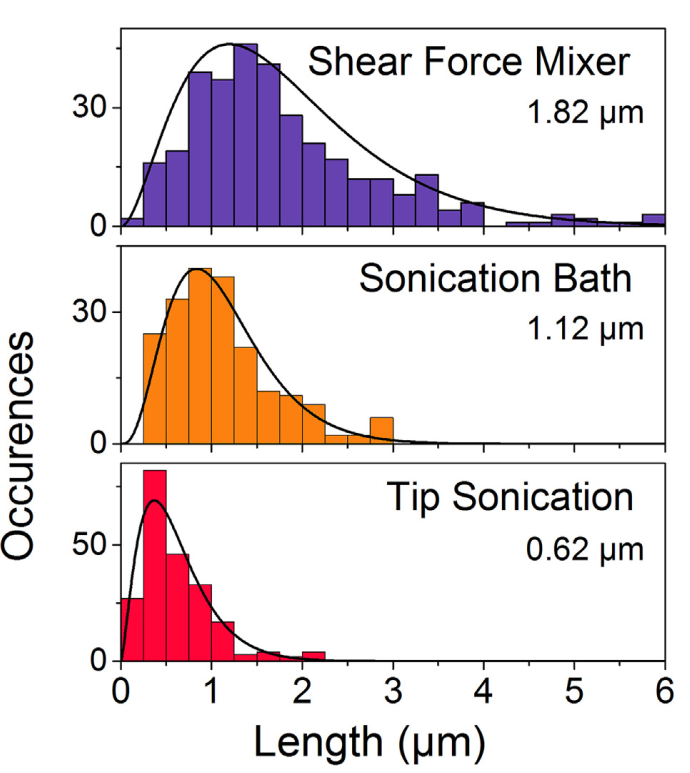
\includegraphics[scale=1.7]{images/chapter_methods/lengths_graf_2}
	\caption{Length distributions, alongside their corresponding average lengths, of (6,5)-enriched ensembles prepared by Graf \textit{et al}.\ \cite{graf2016large} using different dispersion methods. These length distributions were determined using atomic force microscopy. Each sample was prepared using CoMoCAT SWCNTs. For the sample prepared using SFM, the SWCNTs were dispersed in a solution containing toluene and the polymer PFO-BPy. The other samples were obtained by dispersing the SWCNTs in an aqeous solution containing SDS. SFM produced a ensemble of SWCNTs with lengths that were much longer than those obtained by using the other dispersion methods. Reproduced from Ref.\ \cite{graf2016large}.}
	\label{fig:dist_graf}
\end{figure}


\subsection{Chirality Enrichment by Polymer Selection}

Chirality separation of SWCNT ensembles can be also be performed by dispersing SWCNTs in a solution containing aromatic organic polymers \cite{nish2007highly, chen2007toward, tange2011selective}. Here, the polymers selectively solubize certain chiralities of SWCNTs depending on the molecular structures of the polymer and the  SWCNTs \cite{nish2007highly}. This was first demonstrated by Nish \textit{et al}.\ (2007) \cite{nish2007highly}, who studied the optical properties of ensembles that were prepared by dispersing, via sonication and ultracentrifugation, HiPco and CoMoCAT SWCNTs using different polymers in the solvent toluene. They observed that the polymer poly(9,9-dioctylfluorenyl2,7-diyl), commonly referred to as PFO, exhibits a particularly strong selectivity.

Figure \ref{fig:comparison_nish} shows a comparison of the optical absorption spectrum of CoMoCAT SWCNTs ensembles that were dispersed using either an aqeuous solution containing sodium dodeclybenzene sulphonate (SDBS) or a toluene solution containing PFO. The aqueous suspension contains several optical resonances as no chirality separation technique was performed on the sample to enrich any particular nanotube species. In contrast, the polymer-wrapped sample contains fewer and narrower due to the tendency of the PFO polymer to help dissolve only a subset of chiralities within then ensemble. However, Nish \textit{et al}.\ also mentioned that this selectivity only occurred when using toluene as the solvent rather than other organic solvents such as choloroform \cite{nish2007highly}.

\begin{figure}[H]
	\centering
	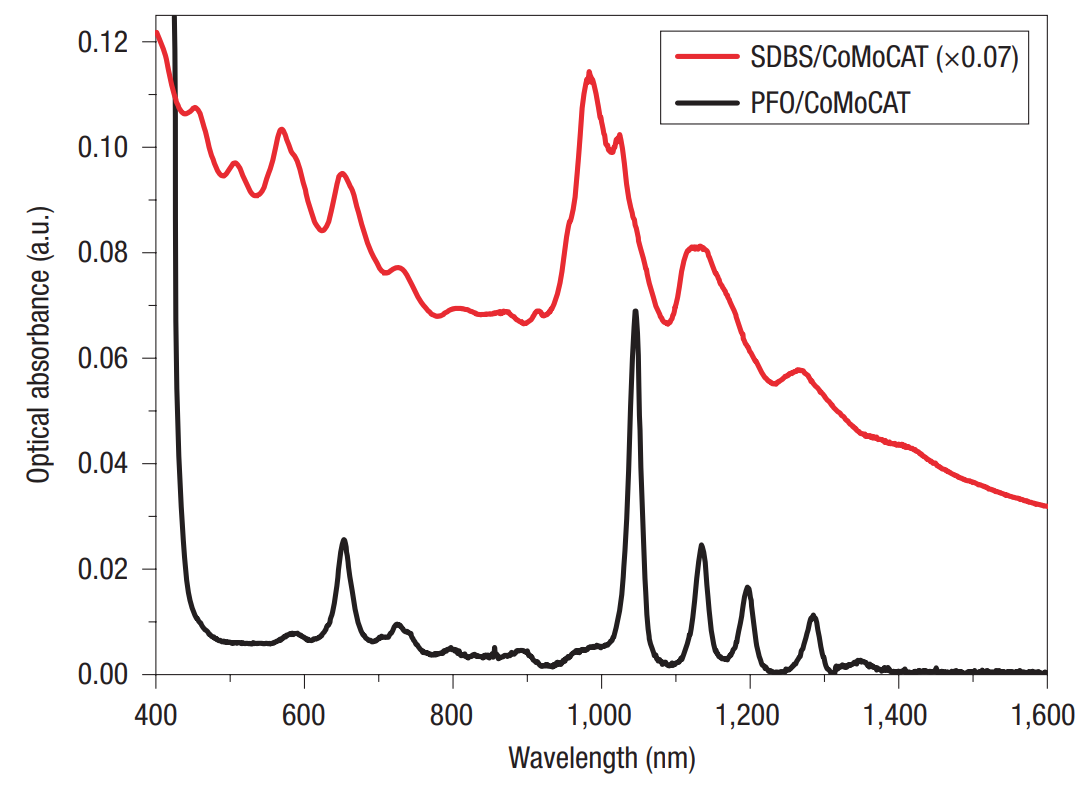
\includegraphics[scale=1.4]{images/chapter_methods/purification_nish_2}
	\caption{Optical absorption spectra for CoMoCAT SWCNTs dispersed in an aqueous SDBS surfactant solution and in a toluene solution containing the polymer PFO. The suspension created using PFO contains fewer and narrower optical resonances due to the tendency of the PFO polymer to suspend only a subset of chiralities in the solution. Reproduced from Ref.\ \cite{nish2007highly}. }
	\label{fig:comparison_nish}
\end{figure}


The mechanism for how these polymers solubize SWCNTs depends on the SWCNT diameter. Nish \textit{et al}.\ conducted molecular dynamics to illustrate this \cite{nish2007highly}. They observed that the polymer structures form around SWCNTs at a fixed distance from the SWCNT surface, as shown in Figure \ref{fig:model_nish}. This differs from the solubization mechanism of surfactants which instead form micelle structures on the SWCNT surface \cite{richard2003supramolecular}. Furthermore, the polymer structures that form around each SWCNT have an $n$-fold symmtery. This means that for a given SWCNT, $n$-polymers will have to be connected in the circumferential direction to suspend the SWCNT in the toluene solution. Nish \textit{et al}.\ revealed that this has a clear diameter dependence \cite{nish2007highly}. For a (6,1) SWCNT, two polymer units will have to be wrapped in around the SWCNT, whereas for a (8,0) SWCNT three polymer units will needed to suspend the SWCNT. They also determined from these simulations that the binding energy of each polymer structure also scales linearly with the SWCNT diameter.

Aside from this, Nish \textit{et al}.\ observed that each polymer selectively interacts with certain chiralities  \cite{nish2007highly}. Figure \ref{fig:map_nish} shows photoluminescence excitation maps for two different HiPco SWCNT ensembles that were suspended using the polymers PFO and PFH (poly[9,9-dihexylfluorenyl-2,7-diyl]). Here, they showed that the ensemble prepared using exhibits a high selectivity for (8,6) SWCNTs given by the relatively higher photoluminescence emission of this chirality. By comparison, the PFH polymer created a suspension enriched by (8,7), (9,7), and (8,6) nanotubes. Both polymers also effectively removed other nanotubes such as (9,1) and (6,5) SWCNTs from the suspension. In other studies, it has been shown that the polymer poly[(9,9-dioctylfluorenyl-2,7-diyl)-alt-co-(6,6 0 -\{2,2 0 -bipyridine\})], commonly abbreviated as PFO-BPy, can be used to create (6,5)-enriched suspensions due to the seletivity of PFO-BPy \cite{hertel2010diffusion, ozawa2011one, gomulya2013conjugated}. This is precisely how our sample was prepared by using this polymer.


\begin{figure}[H]
	\centering
	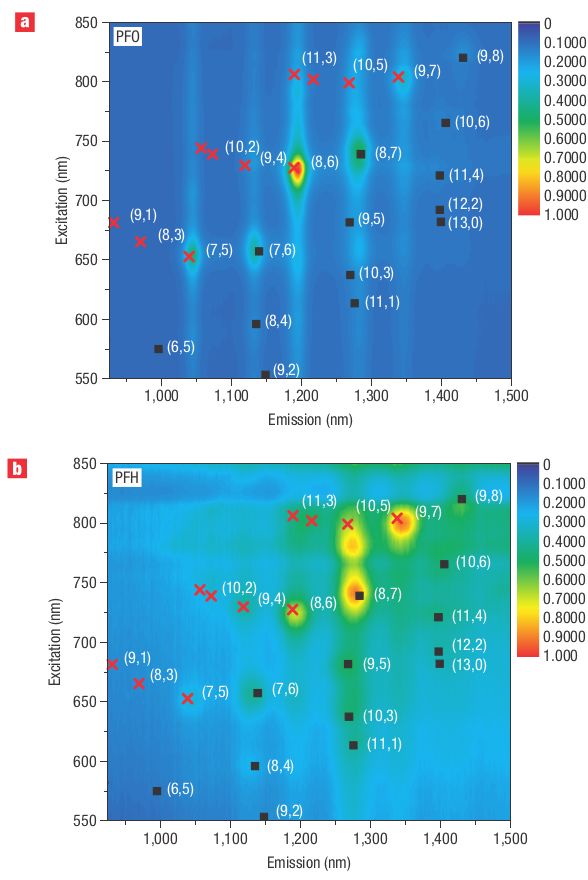
\includegraphics[scale=2.3]{images/chapter_methods/pl_nish_3}
	\caption{Photoluminescence excitation maps of two polymer-SWCNT samples in toluene solutions prepared by Nish \textit{et al}.\ \cite{nish2007highly}. These include SWCNT suspensions prepared using the polymers (a) PFO and (b) PFH. Furthermore, the colorbar scale corresponds to the intensity of the emission. The plots show the differences in the chirality selectivity of the two polymers.
	%Figure \ref{fig:molec_structure_nish} shows the molecular structure of these polymers. Reproduced and modified from Ref.\ \cite{nish2007highly}.
	}
	\label{fig:map_nish}
\end{figure}

\begin{figure}[H]
	\centering
	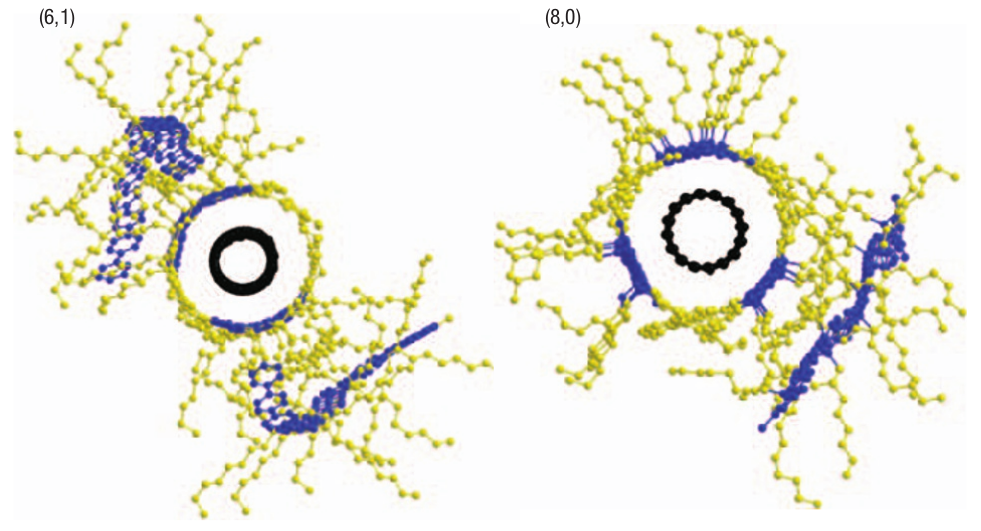
\includegraphics[scale=0.35]{images/chapter_methods/poly_structure_nish}
	\caption{Radial views of PFO polymer structures that form around (6,1) and (8,0) SWCNTs (shown in the center), as presented by Nish \textit{et al}.\ \cite{nish2007highly}. Around the exterior of the SWCNTs, the PFO structures are presented with the polymer backbone presented in blue (dark) and the sidechains presented in yellow (light). These structures form around SWCNTs at a fixed distance from the nanotube surface. Nish \textit{et al}.\ noted that there is a significant diameter dependence in this process. In particular, the polymer structures surrounding the SWCNTs have an $n$-fold symmetry. Depending on the diameter of the SWCNT, these structures can be composed of $n$ polymers bound in the circumferential direction. For the (6,1) SWCNT, two polymer units are involved in solubization, whereas for the (8,0) nanotube, three polymer units are involved. Molecular dynamic simulations also indicated that the binding energy for a given polymer structure tends to scale linearly with the SWCNT diameter. Reproduced from Ref.\ \cite{nish2007highly}.}
	\label{fig:model_nish}
\end{figure}

%\begin{figure}[H]
%	\centering
%	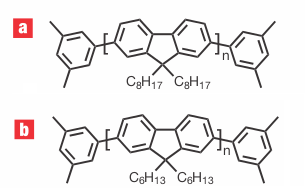
\includegraphics[scale=3]{images/chapter_methods/molecular_structure_nish}
%	\caption{Molecular structures of (a) PFO and (b) PHF. }
%	\label{fig:molec_structure_nish}
%\end{figure}



\subsection{Optical Spectrum of (6,5)-enriched Samples}

Measuring the attenuance of prepared samples provides a means of determining the different chiralities present in the sample as well as their relative populations. Here, attenuance $A$ is defined as
\begin{equation}
A = \log_{10}\left(\dfrac{I_{\mathrm{ref}}}{I_{\mathrm{sample}}}\right),
\end{equation}
where $I_{\mathrm{ref}}$ and $I_{\mathrm{sample}}$ represent the optical transmission through a reference sample and the nanotube sample respectively. In literature, this is also commonly referred to as absorbance. However, the key difference between the terms attenuance and absorbance is that attenuance accounts for losses due to both reflection and scattering whereas absorbance does not \cite{dixon1992absorbance}. The reference sample only contains water and a 4\% concentration of DOC and is also stored in a cuvette with an optical path length of 1 mm.

Figure \ref{fig:sample_absorbance} presents the attenuance spectrum of the (6,5) sample measured using the white-light supercontinuum source described in Section \ref{section:white_light_probe}. The spectrum exhibits a number of optical transitions including the $E_{11}$, phonon sideband, $E_{12}$, and $E_{22}$ resonances at photon energies of 1.26, 1.45, 1.9, and 2.17 eV, respectively. Furthermore, other small peaks in the sample at 1.35 and 1.41 eV emerge from exciton resonances of residual (9,1) and (6,4) nanotubes respectively.

\begin{figure}[H]
	\centering
	\includegraphics[scale=0.7]{example-image-a}
	\caption{ Attenuance spectrum of (6,5) sample measured using the white light source described in Section \ref{section:white_light_probe}. Optical transitions including the $E_{11}$, $E_{11} $ phonon sideband, $E_{12}$, and $E_{22}$ occur at 1.26, 1.45, 1.9 and 2.17 eV respectively. Other peaks at 1.35 and 1.41 eV appear due to a small presence of (9,1) and (6,4) nanotubes in the dispersion.}
	\label{fig:sample_absorbance}
\end{figure}



\section{Experimental Apparatus for Pump-Probe Spectroscopy}
\label{sec:experimental_proced}

%include figure of setup
\subsection{Overview}
The experimental apparatus, illustrated in Figure \ref{fig:setup_schematic}, incorporates the use of an intense optical pump pulse followed by a broadband probe pulse to characterize the ultrafast carrier dynamics of carbon nanotubes. The pump and probe beams are focused onto the surface of the sample in a noncollinear geometry. Here, the probe beam transmits through the sample at normal incidence. However, the pump beam propagates through the sample at an offset angle of \SI{40}{\degree}. Finally, the transmission spectrum of the probe is resolved using a spectrometer to resolve the nonequilibrium optical properties of the sample.


\begin{figure}[ht]
	\centering
	\includegraphics[scale=0.7]{example-image-a}
	\caption{Schematic diagram of the experimental apparatus. The setup is powered by a Ti:sapphire femtosecond laser (Clark-MXR CPA-2010) that generates $\sim$200 fs, 775 nm (1.6 eV) pulses at a repetition rate of 1 kHz and an average power of 1 W. The total laser output is delivered to an optical parametric amplifier (TOPAS-800). The OPA generates a signal (1.1 $-$ \SI{1.5}{\micro\meter}) and idler beams (1.5 $-$ \SI{2.7}{\micro\meter}) using a type-II parametric generation process.  A BBO crystal is mounted at the output of the OPA to generate the second-harmonic of the signal in a type-II process. A wavelength separator containing a set of dichroic mirrors separates the second-harmonic of the signal, used as the optical pump, from the fundamental of the signal used to generate the white light supercontinuum probe.}
	\label{fig:setup_schematic}
\end{figure}


\subsection{Chirped Pulse Amplifier}
The CPA-2010 laser source manufactured by Clark-MXR functions as the heart of this optical setup. It operates with a repetition rate of 1 KHz and outputs pulses with a 200 fs duration, a central wavelength of 775 nm, and a pulse energy of 1 mJ. This laser generates amplified pulses using a chirped pulse amplification process illustrated in Figure \ref{fig:cpa_process}.

Chirped pulse amplification makes it possible to amplify ultrashort pulses without incurring the risk of damaging optical components due to self-focusing effects \cite{strickland1985compression}. This is done by first stretching a relatively weak, short pulse, also known as the seed pulse, by inducing dispersion with a pair of gratings. Next, the stretched pulse enters a gain medium that amplifies the intensity of the stretched pulse. Without the initial stretching step, the intensity of the amplified seed pulse may exceed the damage threshold of the optical components in the laser such as the gain medium. Afterward, the pulse is compressed by another pair of gratings before exiting the laser cavity.

\begin{figure}[ht]
	\centering
	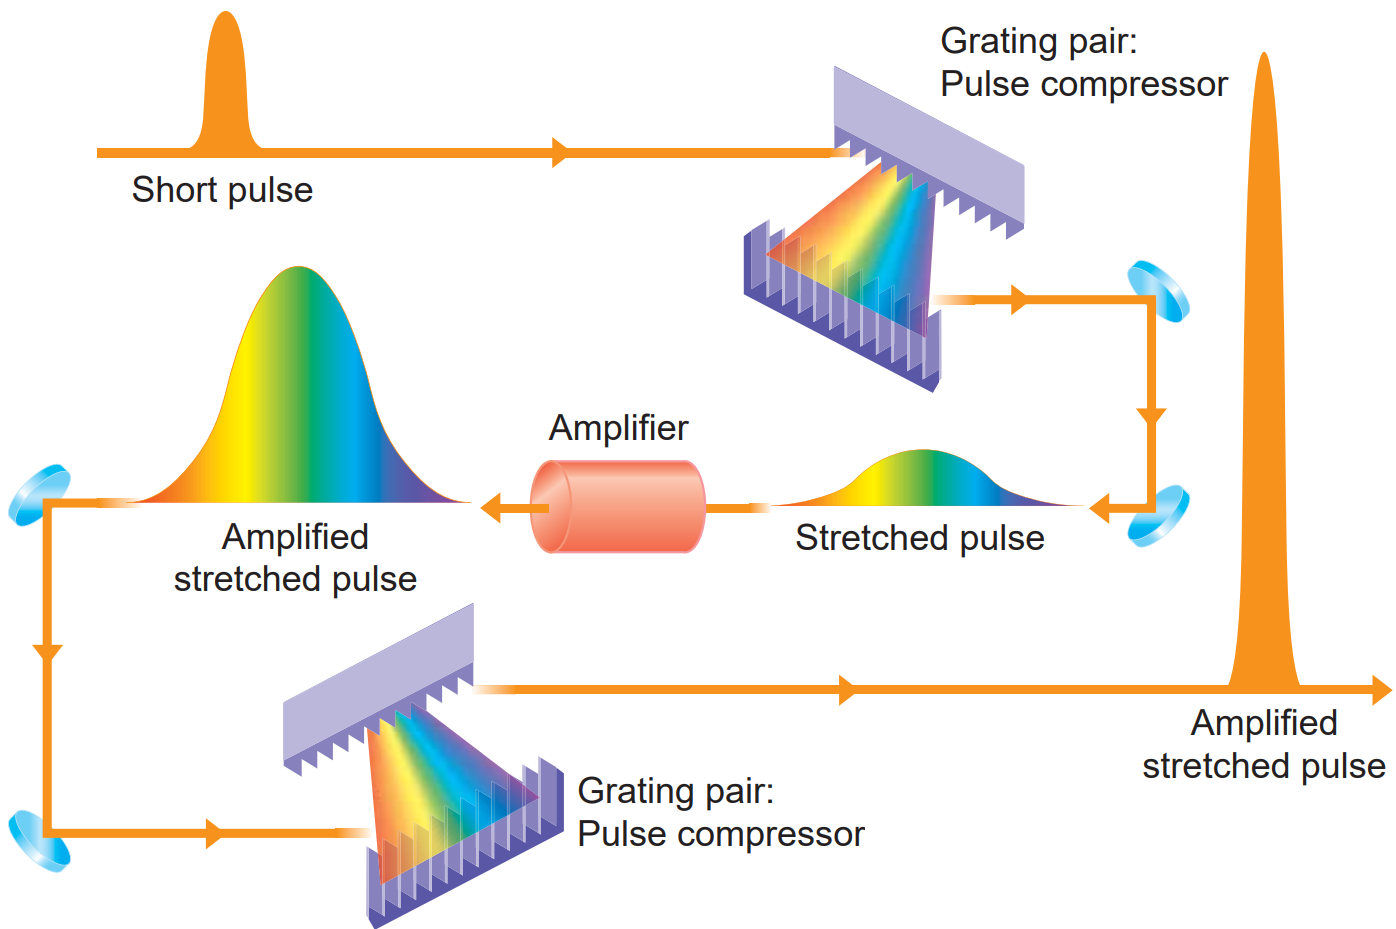
\includegraphics[scale=0.31]{images/chapter_methods/cpa_process_service}
	\caption{Schematic diagram of the chirped pulse amplification process. A short pulse is initially stretched by a pair of gratings, amplified by the system, and then recompressed to yield an amplified short pulse. Reproduced from Ref.\ \cite{service154}.}
	\label{fig:cpa_process}
\end{figure}

The CPA-2010 utilizes a laser oscillator to generate seed pulses. This oscillator features a single-mode erbium-doped fiber (SErF), which serves as the gain medium that is pumped by a solid-state fiber-coupled laser operating at 980 nm. In addition, the oscillator generates pulses with a central wavelength of 775 nm at a repetition rate of 30 MHz. Finally, the seed pulse is stretched in time by a transmission grating before entering the regenerative amplifier for the amplification step.

The regenerative amplifier system uses a Ti:sapphire crystal as its gain medium that is optically pumped by the frequency-doubled output of a Nd:YAG (neodymium-doped yttrium aluminum garnet; Nd:Y$_3$Al$_5$O$_{12}$) laser cavity. The Nd:YAG laser cavity uses a Nd-doped YAG crystal as its gain medium and a KTP (potassium titanyl phosphate; KTiOPO$_4$) crystal to frequency-double its output. Furthermore, it outputs nanosecond-duration pulses, centered at 532 nm, at a repetition rate of 1 kHz.

A Pockels cell driver dictates when a seed pulse from the oscillator can enter the regenerative amplfier cavity as well as when the amplified seed pulse can exit the cavity. Correspondingly, it also synchronizes the timing of the pump pulse from the Nd:YAG cavity and the seed pulse to ensure that they arrive at the Ti:sapphire crystal at the same time. In total, the amplified seed pulse undergoes 5 roundtrips through the regenerative amplifier. Afterwards, the amplified seed pulse passes through a transmissive grating of the pulse compressor four times and is compressed to down to a pulse duration of 200 fs before being ejected as laser output.

\subsection{Optical Parametric Amplifier}
\label{section:opa}

The optical parametric amplifier (OPA) used in the setup is a TOPAS-800 produced by Light Conversion \cite{topas}. It produces pulses of $\sim$200 fs duration at a repetition rate of 1 kHz, just like the CPA, but with a lower average power that can be as high as \SI{200}{\milli\watt} depending on the selected wavelength of the emission. In fact, this tunable light source can generate radiation in the range of \SI{530}{\nano\meter} $-$ \SI{20}{\micro\meter}. The OPA relies on conducting parametric generation processes to achieve this feat.

In the first step, the OPA focuses a small part of the CPA pump beam into a barium borate (BBO) crystal to generate a white light supercontinuum (see Section \ref{section:white_light_probe}). A small spectral region of the white light, also known as the signal beam of frequency $\omega_\text{signal}$, is selected using a reflective diffraction grating and amplified in the following step. In the final stage, both the amplified signal beam along with the remainder of the CPA pump beam travel through the BBO crystal together. Here, parametric generation occurs in a type-II phase-matching process where an idler beam of frequency $\omega_\text{idler}$ is produced such that
\begin{equation}
	\omega_\text{idler} = \omega_\text{CPA} - \omega_\text{signal}.
\end{equation}
\cite{dunn1999parametric, boyd2003nonlinear}.

The signal and idler wavelengths can take wavelengths of 1.1 $-$ 1.5 $\mu$m  and 1.5~$-$~2.7 $\mu$m, respectively, depending on the alignment of the grating. An additional BBO crystal placed at the output of the OPA provides a means of generating the second harmonic of the signal or idler, which can be used to access wavelengths \SI{530}{nm} $-$ \SI{1}{\micro \meter} via type-II phase matching as well. Alternatively, a different nonlinear crystal such as gallium selenide (GaSe) can be placed at the output for difference-frequency generation (DFG) that generates a beam of frequency $\omega_\text{DFG}$ where
\begin{equation}
	\omega_\text{DFG} = \omega_\text{signal} - \omega_\text{idler}
\end{equation}
to generate wavelengths in the range 2.7 $-$ \SI{20}{\micro\meter}.
\subsection{Filters}

The setup features a wavelength separator that seperates the fundamental of the signal (FS) from the second harmonic of the signal (SHS). This optical device contains a set of two dichroic mirrors that reflect the SHS and transmit the FS. As a result of the type-II second harmonic generation process used to generate the SHS, the polarization of SHS remains perpendicular to that of FS. Hence, a half-wave plate is placed in the optical path of the SHS and appropriately adjusted to make the polarizations of FS and SHS parallel to each other. In addition to this, two neutral density wheels are used to attenuate the intensity of the probe and the optical pump.

\subsection{White Light Continuum Probe}

\label{section:white_light_probe}
Supercontinuum generation represents a nonlinear optical process by which the spectrum of an incident laser pulse becomes significantly broadened \cite{alfano1970emission, alfano1970observation, alfano1989supercontinuum, dubietis2017ultrafast}. It has been observed to occur in many different media such as water, fused silica, sapphire and calcium fluoride \cite{alfano1989supercontinuum, dubietis2017ultrafast}. This process is facilitated by the formation of a filament, which starts as a result of self-focusing \cite{alfano1989supercontinuum, dubietis2017ultrafast}. In other words, the refractive index of the supercontinuum generation medium depends on the intensity of propagating light \cite{alfano1989supercontinuum, dubietis2017ultrafast}. Due to the interplay between this self-focusing and other competing effects such as self-phase modulation, and multiphoton absorption, the spectrum  broadens as the pulse travels through the medium \cite{alfano1989supercontinuum, dubietis2017ultrafast}.

\begin{figure}[ht]
	\centering
	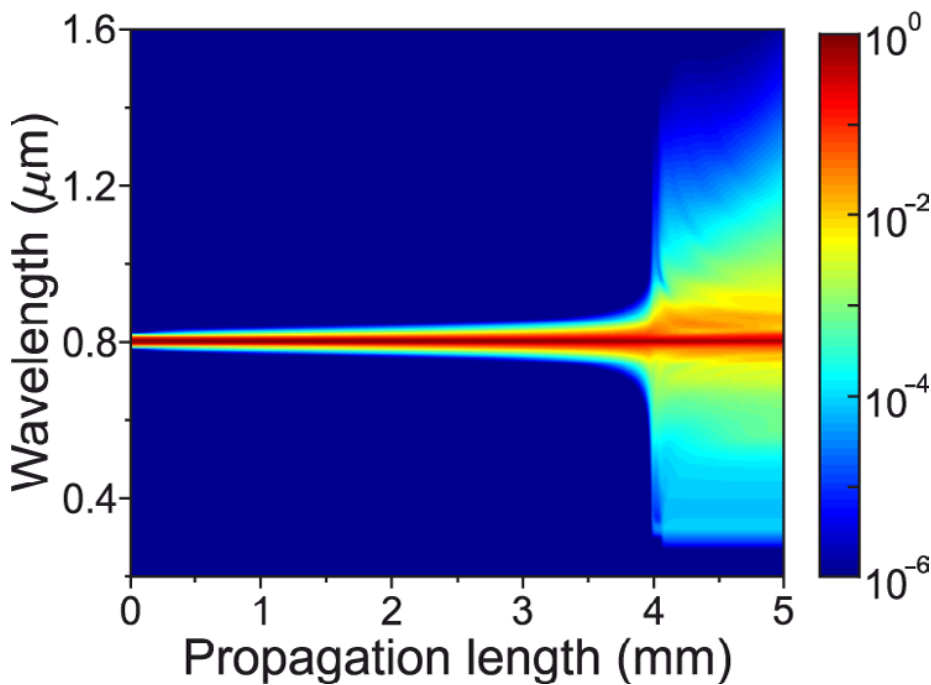
\includegraphics[scale=0.4]{images/chapter_methods/sc_gen_dubietis}
	\caption{Numerical simulation of supercontinuum generation conducted by a 100~fs pulse of wavelength 800 nm. The plot shows how the spectral broadening of the incident pulse evolves as it propagates through a sapphire crystal. The colorbar corresponds to intensity. Reproduced and modified from Ref.\ \cite{dubietis2017ultrafast}.}
\end{figure}
In our setup, supercontinuum generation occurs by focusing (focal length of 6 inches) the fundamental of the signal beam (FS) into a sapphire crystal with a thickness of 5 mm. Here, the center of the sapphire crystal is placed at a distance of one focal length of the lens used to focus the FS. This process generates a white-light continuum that spans 1 $-$ 2.4 eV.

Finally, an iris is placed in the path of FS such that its aperture is positioned at the center of the FS beam. This iris is used to crop the outer portion of the FS, thereby reducing its beam diameter. Doing this has been observed to have the effect of minimizing the temporal fluctuations of the generated white light spectrum. The main strategy for optimizing the stability of the white-light generation is to monitor the white-light spectrum using a spectrometer (Section \ref{section:spectrometer}) whilst adjusting, through trial and error, the distance of the sapphire crystal to the focusing lens as well as the aperture of the iris used to crop the FS.

\subsection{Motorized Delay Stage and Optical Shutter}

The setup includes a motorized delay stage and an optical shutter that are used to control the pump conditions in each measurement. The delay stage consists of a pair of retro-reflecting mirrors mounted on a motorized stage. These mirrors are aligned such that the pump beam's direction of propagation is parallel to that of the motorized stage's direction of motion. The pump beam travels to both of these mirrors. Hence, adjusting the position of the motorized stage alters the time delay between the pump and probe pulses by either increasing or decreasing the optical path length traveled by the pump pulse.

The optical shutter makes it possible to block the pump beam in order to measure probe transmission through the sample under equilibrium conditions. At each time delay, the transmission of the probe beam is measured with the pump beam blocked and with the pump beam unblocked by the shutter. Conducting measurements in this manner mitigates the effect of long-term fluctuations in the laser output.

\subsection{Spectrometer}
\label{section:spectrometer}
The probe is collected into an optical fiber, which sends the probe beam to a SpectraPro 300i$^{\tiny \textregistered}$ spectrometer built by Princeton Instruments.  The spectrometer uses a grating with a diffraction grating with a blaze wavelength of 800 nm and a groove density of 150 grooves per mm. The diffracted light is then imaged onto a charge-coupled device (CCD) camera to measure the probe spectrum.

The camera is silicon-based and contains an array of 1340 $\times$ 100 pixels. It must be cryogenically cooled to a temperature of \SI{-100}{\celsius} using liquid nitrogen for an optimal signal-to-noise ratio.


\section{Measurement of Pump and Probe Spot Size}
\label{section:spot_size}
The pump and probe spot sizes are measured using a knife edge scan technique \cite{firester1977knife}. For this, a razor blade attached to a post is mounted on a motorized stage placed in the sample position. The sharp edge of the blade faces in a direction perpendicular to that of the direction of propagation of the incident beam. A power meter is placed behind the razor blade to measure the average power of the transmitted beams.

\begin{figure}[ht]
	\centering
	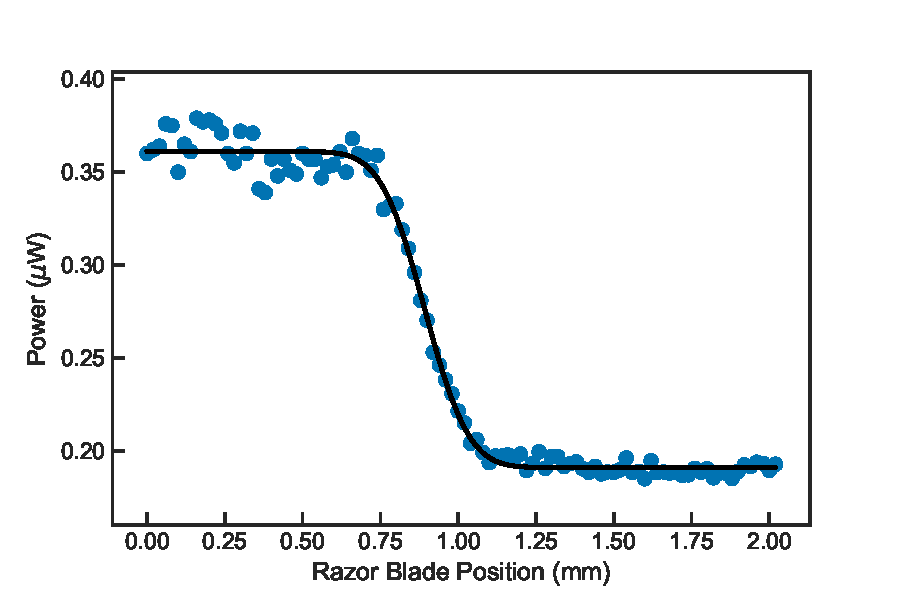
\includegraphics[scale=0.65]{images/chapter_methods/probe_spot_size}
	\caption{Spot size measurement of the white light probe at the sample position. The solid line is a fit to the data using Equation \ref{eq:cdf_gauss}. The fitting yields a beam diameter of 180 $\pm$ \SI{10}{\micro\meter}. }
\end{figure}


As the motorized stage moves the razor blade's position laterally with respect to the beam's propagation direction, the razor blade increasingly blocks portions of the incident beam.  Measuring the transmitted power of the incident beam as a function of razor blade position yields a cumulative distribution function of the incident light's intensity.

\begin{figure}[ht]
	\centering
	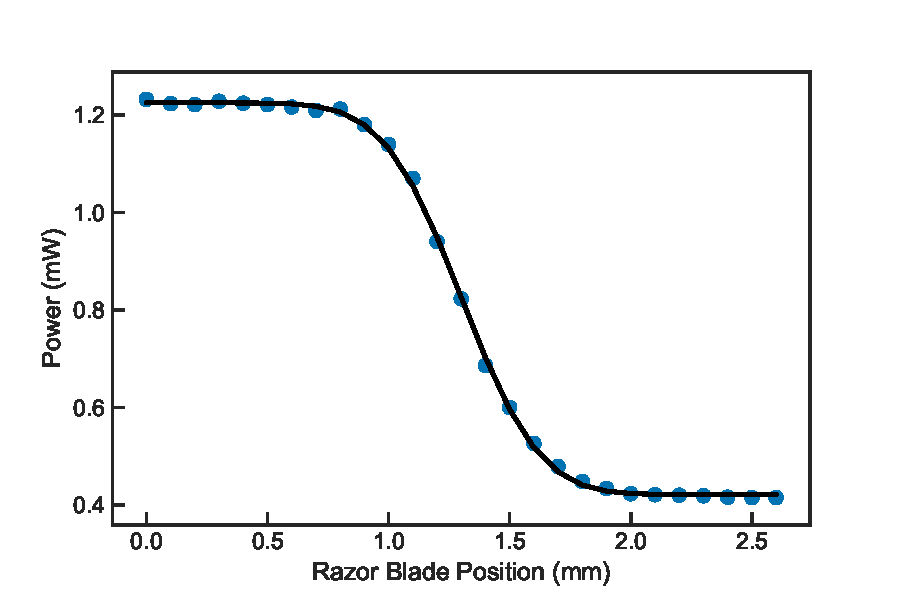
\includegraphics[scale=0.65]{images/chapter_methods/pump_spot_size}
	\caption{Spot size measurement of the 570 nm optical pump at the sample position. The solid line is a fit to the data using Eq.\ \ref{eq:cdf_gauss}. The fitting yields a beam diameter of 550 $\pm$ \SI{9}{\micro\meter}.}
\end{figure}

Assuming that the beam diameter can be approximated as a Gaussian function, the spot size can be estimated by fitting this data with the equation
%
\begin{equation}
	\label{eq:cdf_gauss}
	P = P_0 + \dfrac{P_{\mathrm{max}}}{2} \left\{ 1 - \mathrm{erf} \left( \dfrac{\sqrt{2}(x - x_0)}{w} \right) \right\},
\end{equation}
%
which represents the cumulative distribution function of a Gaussian function. This function yields the beam diameter $w$. Furthermore, $P_0$ represents the baseline of the power meter observed when the beam is fully blocked, erf stands for the standard error function, $P_\text{max}$ denotes the maximum power of the beam, $x$ parametrizes the position of the blade and $x_0$ indicates the position at which the blade blocks 50\% of the incident beam's average power.

\section{Pulse Duration Characterization}
\label{section:pulse_duration}

We used an intensity autocorrelation technique to characterize the pulse duration of laser pulses generated by the CPA-2010 and the OPA \cite{paschotta2008field}. For this, the laser beam of interest is split into two arms using a beam splitter, where one arm is temporally delayed using a delay stage. Both beams are spatially and temporally overlapped on a BBO crystal. Under these conditions, a third beam is generated in the crystal as a result of sum-frequency generation, otherwise referred to as the autocorrelation signal $I_\text{ac}$ defined as
%
\begin{equation}
	I_\text{ac}(\tau) = \int\displaylimits_{-\infty}^{\infty} P_1(t)P_2(t+\tau) \text{d}t
\end{equation}
%
that depends on the time-dependent power of the two incident beams $P_1(t)$ and $P_2(t)$ as well as the temporal delay $\tau$ between them. Assuming that the pulse's temporal profile obeys a Gaussian function, the experimental data can be fit to the expression
%
\begin{equation}
	F(\tau) = \mathrm{ exp}\left[ - \left( \dfrac{2\tau\sqrt{\ln (2)}}{1.41 \Delta t_\text{p}} \right)^2\right]
	\label{eq:pulse_duration_fit}
\end{equation}
%
to estimate the pulse duration $\Delta t_\text{p}$. Figures \ref{fig:cpa_autocorr} and \ref{fig:opa_autocorr} show the experimental data obtained from the CPA and OPA pulses.

Note, however, that the results of this measurement are highly sensitive to the alignment of the compressor in the CPA-2010. Here, the dispersion of the outgoing pulses of the CPA can be tuned by adjusting the position of a right-angle mirror mounted on a translation stage. This right-angle mirror is used in conjunction with a prism to enable the temporally-stretched, amplified seed beam (AS) to complete a total of four passes through a transmissive grating in the pulse compression process.

After exiting the amplifier system, the AS is diffracted by a transmissive grating and now propagates toward the right-angle mirror. This mirror sends the AS back toward the transmissive grating in a path parallel to AS's incident direction of propagation to complete the second pass. This time, the grating sends the AS to a prism which elevates the AS and sends it back to the grating. The AS now traverses through the grating a third time. Here, the grating sends the AS back to the right-angle mirror, which reflects it toward the grating to complete the fourth pass. By moving the mirror in a direction parallel to the amplified seed beam's incident direction of propagation, this adjusts the total path length traveled by the amplified seed beam inside the compressor and therefore modulates the beam's dispersion.

%\begin{figure}[ht]
%	\centering
%	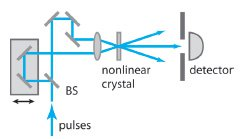
\includegraphics[scale=0.7]{images/chapter_methods/autocorrelator}
%	\caption{Reproduced from \cite{paschotta2008field}.}
%\end{figure}

\begin{figure}[ht]
	\centering
	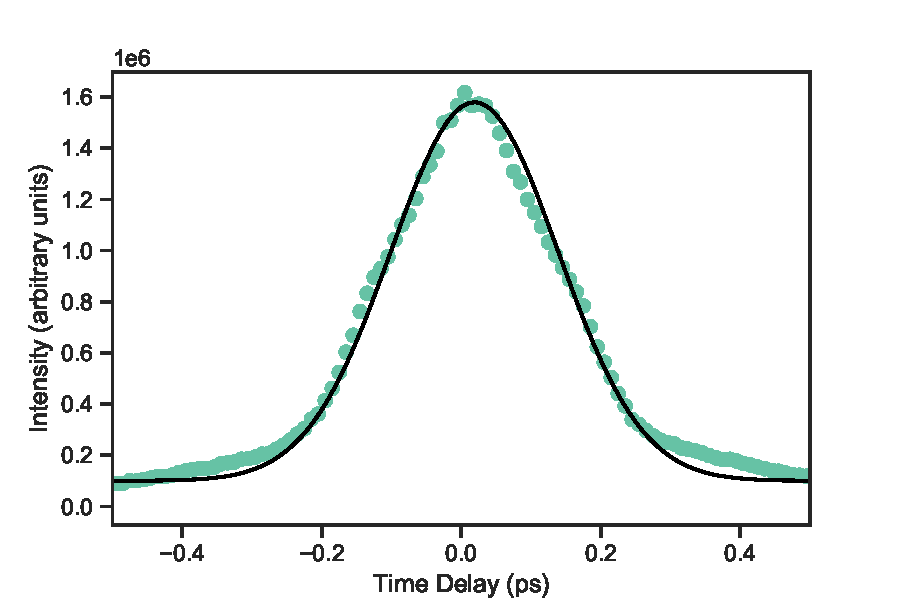
\includegraphics[scale=0.6]{images/chapter_methods/cpa_autocorr}
	\caption{Autocorrelation signal of the CPA-2010 output. The solid line corresponds to a fit to the data using Eq.\ \eqref{eq:pulse_duration_fit}. Curve-fitting yields a pulse duration of $\sim$200 fs.}
	\label{fig:cpa_autocorr}
\end{figure}

\begin{figure}[ht]
	\centering
	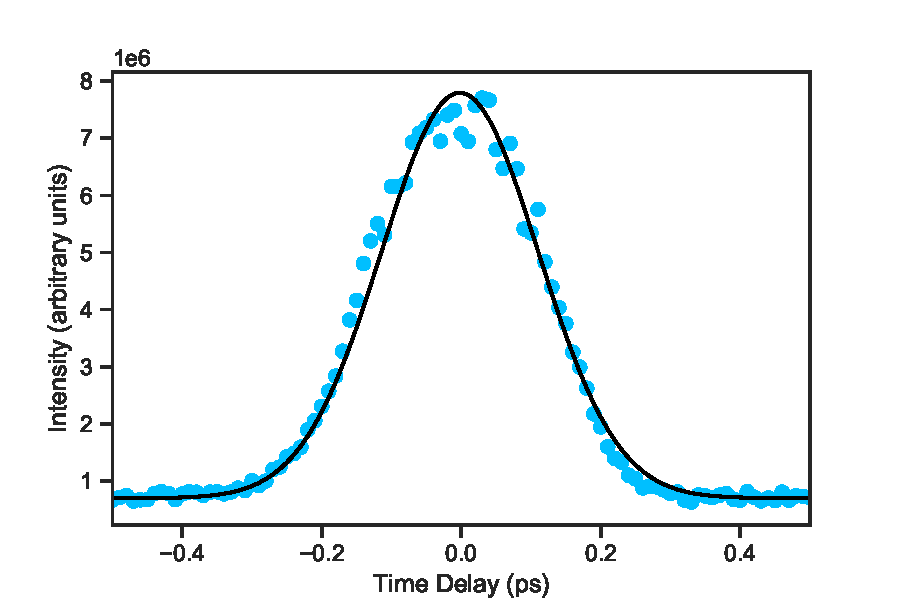
\includegraphics[scale=0.6]{images/chapter_methods/opa_pump_autocorr}
		\caption{Autocorrelation signal of the OPA signal output set to 1190 nm. The solid line corresponds to a fit to the data using Eq.\ \eqref{eq:pulse_duration_fit}. Curve-fitting yields a pulse duration of $\sim$190 fs.}
		\label{fig:opa_autocorr}
\end{figure}

\section{Fluence, Peak Power, and Power Density}
In pump-probe spectroscopy, the terminologies fluence (J/cm$^2$), peak power (W), and power density (W/cm$^2$) are commonly used to describe the strength of the optical pump. The fluence $F$ defined as
\begin{equation}
	F \equiv \dfrac{P_\text{avg}}{f} \dfrac{1}{\pi r^2} = \dfrac{E}{\pi r^2}
\end{equation}
takes into account the pulse energy of the pump $E$, as well as the pump beam's cross-sectional radius $r$. Here, $E$ represents the average power of the pump $P_\text{avg}$ divided by the repetition rate of the laser $f$. The parameters $P_\text{avg}$ and $r$ can both be obtained via the knife-edge scan method defined in Section \ref{section:spot_size}.

In contrast, the peak power $P_\text{peak}$ and the power density $I_\text{p}$ both account for the pulse duration $\Delta t_\text{p}$ of the pump pulse that can be obtained in the autocorrelation method described in Section \ref{section:pulse_duration}. More specifically, the peak power is defined as
\begin{equation}
	P_\text{peak} \equiv \dfrac{E}{\Delta t_p}
\end{equation}
whereas, the power density is given as
\begin{equation}
	I_\text{p} \equiv \dfrac{E}{\pi r^2 \Delta t_\text{p}} = \dfrac{P_\text{peak}}{\pi r^2} =\dfrac{F}{\Delta t_\text{p}}.
\end{equation}
Amongst these definitions, the power density is more comprehensive as it includes both spatial and temporal information of the optical pump pulses.
